\chapter{Architettura Hardware dello strumento}
\label{capitolo3}
\thispagestyle{empty}

\textit{In questo Capitolo verrà descritta l'architettura hardware dello strumento realizzato. Prima verrà analizzata brevemente la parte analogica dello strumento. Successivamente verrà descritta la parte di conversione analogico-digitale e digitale-analogico soffermandoci prima sulle architetture dei convertitori presenti in letteratura e poi su quelle presenti nello strumento. Infine verrà presentata la parte digitale motivando la scelta dell'uso di una scheda di prototipazione contenente FPGA e microcontrollore.}

\section{Struttura complessiva dello strumento}
Lo strumento di misura progettato in questo elaborato è un misuratore \textit{contactless} di distanza. Lo scopo è realizzare un sistema \textit{embedded} in grado di gestire in modo autonomo tutta la misura, dal controllo della sorgente laser all'acquisizione ed elaborazione del segnale interferometrico.

Per sistema \textit{embedded}, si intende un sistema di elaborazione progettato appositamente per una specifica applicazione (\textit{special purpose}). Come già introdotto, l'applicazione in questione è la misura di distanza. 

Il principio fisico per il quale è possibile effettuare una misura è stato descritto nel Capitolo \ref{capitolo2}.
\begin{figure}  
  \begin{center}
  %%TODO Cap3: Foto finale dello strumento
    %\includegraphics[scale=0.5]{}
    \caption{Risultato finale del misuratore realizzato}
    \label{fotorisfin}
  \end{center}
\end{figure}\\
La Figura \ref{fotorisfin} mostra il risultato finale del misuratore progettato e realizzato per questo lavoro di Tesi. Dalla figura si possono distinguere le tre parti principali che compongono lo strumento:
\begin{itemize}
	\item \underline{Parte analogica}: La parte analogica è costituita da una sezione ottica e una sezione analogica. La sezione ottica è composta dal package della sorgente laser, che comprende laser, fotodiodo e lente collimatrice. La sezione analogica comprende il circuito di alimentazione del laser e gli stadi di condizionamento e amplificazione del segnale interferometrico generato dal fotodiodo.
	\item \underline{Parte di conversione}: La parte di conversione è formata da due sezioni: la sezione di conversione analogico-digitale (ADC) e la sezione di conversione digitale-analogico (DAC). La prima sezione provvede ad effettuare la conversione analogico-digitale del segnale interferometrico in uscita dalla parte analogica. Mentre, la seconda sezione effettua la conversione digitale-analogica dal segnale di modulazione del laser in uscita dalla parte digitale.
	\item \underline{Parte digitale}: La parte digitale è costituta da un dispositivo \textit{embedded} di prototipazione composto da un microprocessore e un FPGA. I compiti principali della parte digitale sono la generazione del segnale di modulazione del laser, l'elaborazione del segnale interferometrico per l'estrazione della frequenza di frangia e il calcolo della misura di distanza. Un computer è collegato con la parte digitale tramite connessione \textit{Ethernet}, attraverso questo collegamento è possibile la comunicazione con gli elementi programmabili del sistema.
\end{itemize}
\begin{figure}  
  \begin{center}
    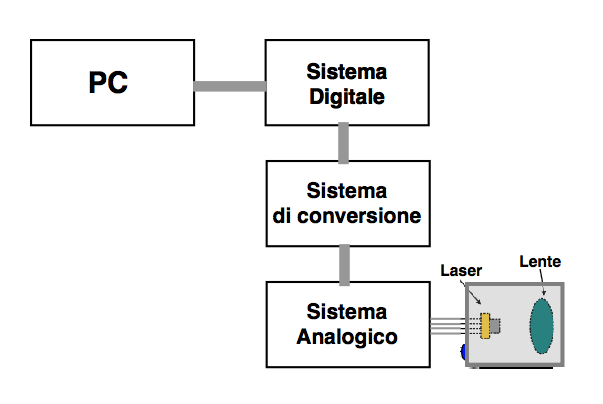
\includegraphics[scale=0.4]{cap3/archgen}
    \caption{Schema a blocchi dell'architettura complessiva del misuratore}
    \label{archgen}
  \end{center}
\end{figure}

L'architettura complessiva del sistema progettato è schematizzata in Figura \ref{archgen}. La Figura mostra lo schema concettuale dello strumento, evidenziando le singoli parti e le connessioni fra quest'ultime.

Nei paragrafi successivi verrà fornita un'analisi dettagliata delle singoli parti dello strumento.

\section{Parte analogica}
La parte analogica è formata da due sotto-sistemi:
\begin{enumerate}
	\item Sistema ottico e sorgente laser
	\item Circuito di interfacciamento con il modulo laser
\end{enumerate}

\subsection{Sistema ottico e sorgente laser}
In lavori precedenti sono state provate diverse sorgenti~\cite{thesispallsilv}~\cite{thesisstorti}. Tra queste è stato scelto il modulo laser \textit{WLSD-1550-020m-1-PD}.
\begin{figure}  
  \begin{center}
    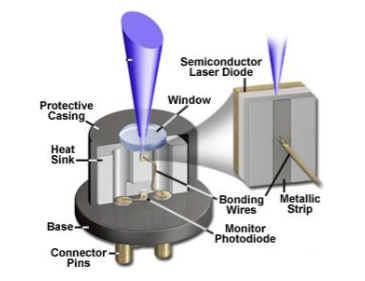
\includegraphics[scale=0.5]{cap3/laserwave}
    \caption{Struttura del dispositivo \textit{WLSD-1550-020m-1-PD}}
    \label{laserwave}
  \end{center}
\end{figure}

Si tratta di una sorgente laser di tipo DFB (\textit{Distributed FeedBack}) prodotta dalla \textit{Wavespectrum}, la cui struttura è mostrata in Figura \ref{laserwave}. Essa emette ad una lunghezza d'onda di $1550nm$.

La sorgente è allineata alla lente per la collimazione, questi due componenti alloggiano in un supporto di alluminio. La lente, codice prodotto \textit{C230TMD-C} realizzata da \textit{Thorlabs}, ha la funzione di raccogliere tutto il fascio laser della sorgente focalizzandolo a piacere. \'E possibile infatti regolarne la posizione avvitandola o svitandola.

Di seguito vengono riassunti i punti chiave che hanno portato alla scelta di tale sorgente laser:
\begin{itemize}
	\item Possiede un buon rapporto segnale/rumore
	\item \'E facile modularne la lunghezza d'onda
	\item Essendo un laser DFB riflette solo una banda ristretta di lunghezze d'onda
	\item Ha un costo accessibile
	\item Appartiene alla classe di sicurezza $1$
	\item Ha una debole riflettività dello specchio permettendo così una forte sensibilità alla retroiniezione
\end{itemize}

Tale sorgente però, emettendo nel non visibile, rende complicati i processi di allineamento.
\begin{figure}  
  \begin{center}
    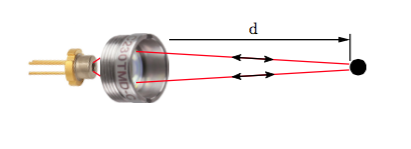
\includegraphics[scale=0.5]{cap3/sistottico}
    \caption{Sistema ottico con laser e lente}
    \label{sistottico}
  \end{center}
\end{figure}
In figura \ref{sistottico} è mostrato il sistema ottico senza supporto. Il bersaglio è schematizzato con un pallino nero e $d$ è la distanza misurata.

\subsection{Circuito di interfacciamento}
Come ampiamente descritto nel Capitolo precedente, è necessario generare una corrente di modulazione sovrapposta a quella di polarizzazione per il diodo laser. Per tale motivo, questo circuito si occupa dell'elaborazione dei segnali analogici, rispettivamente della corrente di pilotaggio del laser e della corrente di uscita dal fotodiodo.
\begin{figure}  
  \begin{center}
    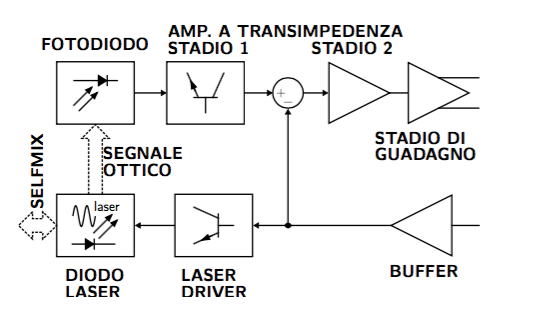
\includegraphics[scale=0.5]{cap3/circanalog}
    \caption{Schema a blocchi del circuito di interfacciamento}
    \label{circanalog}
  \end{center}
\end{figure}

Lo schema logico del circuito è mostrato in Figura \ref{circanalog}. 

Il segnale di modulazione proveniente dalla parte di conversione attraversa un circuito di filtraggio e viene convertito in corrente (corrente di pilotaggio del laser).
Il segnale di corrente dovuto all'effetto interferometrico è minore di $2 \mu A$ , molto più ampio invece è quello associato alla modulazione (circa $1mA$). Per poter estrarre solamente il segnale interferometrico si effettua quindi una differenza del segnale totale rilevato con quello di modulazione del laser. Infine, il risultato della differenza è ulteriormente amplificato e reso disponibile alla parte di conversione in formato differenziale.

Una descrizione più dettagliata della parte analogica e dell'attività di progetto del sistema è trattata nel lavoro di tesi sviluppato dal laureando Samuele Disegna con cui abbiamo collaborato~\cite{thesissmldis}.

\section{Parte di Conversione}
La scheda utilizzata per la parte di conversione del misuratore è la \textit{SCO Board}, progettata e prodotta nel laboratorio di "Misure Ottiche ed Elettroniche - MOLES" del Politecnico di Milano. Anch'essa è stata progetta e realizzata da Samuele Disegna nel contesto del suo lavoro di tesi.
\begin{figure}  
  \begin{center}
    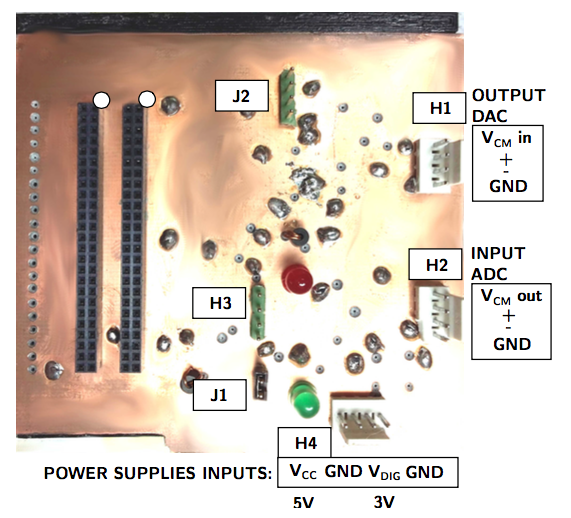
\includegraphics[scale=0.35]{cap3/scoboardfoto}
    \caption{Foto della scheda di conversione \textit{SCO Board} e identificazione delle connessioni}
    \label{scoboardfoto}
  \end{center}
\end{figure}

Essa possiede due interfacce di conversione: un'interfaccia Analogico-Digitale (AD), che riceve in ingresso il segnale interferometrico in arrivo dalla sorgente laser, e un'interfaccia Digitale-Analogica (DA), che converte il segnale digitale di modulazione in arrivo dalla scheda di prototipazione. Le conversioni AD e DA vengono svolte in parallelo.
\begin{figure}  
  \begin{center}
    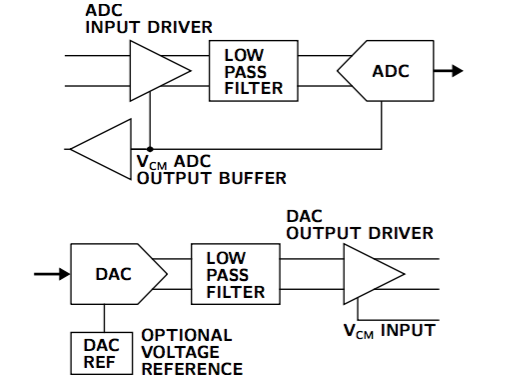
\includegraphics[scale=0.4]{cap3/scoboardschema}
    \caption{Schema a blocchi del sistema di conversione A/D - D/A, \textit{SCO Board}}
    \label{scoboardschema}
  \end{center}
\end{figure}

Le specifiche fornite per la frequenza massima di campionamento dei segnali sono $50MS/s$ con $12$ bit di quantizzazione, essi garantiscono di avere una buona dinamica di misura della distanza e una buona dinamica di ampiezza del segnale misurato con rumore di quantizzazione trascurabile. In Figura \ref{scoboardfoto} e \ref{scoboardschema} sono mostrate rispettivamente la \textit{SCO Board} e il relativo schema a blocchi del circuito.

I due amplificatori operazionali completamente differenziali si occupano della gestione dei segnali analogici. Uno pilota l'uscita differenziale corrispondente al DAC e porta la dinamica di uscita a $1V_{pp}$, l'altro prepara il segnale di ingresso differenziale per il campionamento. I filtri passa basso svolgono la funzione di antialiasing per l'ADC e di ricostruzione del segnale del DAC.

I convertitori presenti sulla \textit{SCO Board} e le loro caratteristiche fondamentali verranno descritte in dettaglio nei paragrafi successivi.

Invece, una descrizione più dettagliata del circuito è fornita in letteratura~\cite{thesissmldis}.

\subsection{Convertitori}
I convertitori Digitale-Analogico (DAC) e Analogico-Digitale (ADC) fanno parte della famiglia dei convertitori dati (\textit{Data Converters}).

Le caratteristiche fondamentali di un convertitore dati sono:
\begin{itemize}
	\item \underline{Risoluzione}: Descrive il numero di valori (livelli di quantizzazione) che il convertitore riesce a distinguere. L'unità di misura è il numero di bit $n$. I livelli di quantizzazione $N$ sono definiti come:
	\begin{equation}
		N=2^n
	\end{equation}
	\item \underline{Dinamica}: Descrive la massima ampiezza del segnale analogico. L'unità di misura è il volt $[V]$.
	\item \underline{Tempo di conversione}: Indica il tempo impiegato dal convertitore per eseguire la conversione. I tempi impiegati per la conversione differiscono notevolmente a seconda della tipologia di convertitore utilizzato, anche se, in generale, la conversione DA è più veloce dell'operazione inversa. Di solito è più conveniente specificare il numero di campioni che possono essere convertiti in un secondo, piuttosto che il tempo di conversione. Tale grandezza è chiamata frequenza di campionamento (o \textit{sampling rate}) e si esprime in Hertz $[Hz]$ o campioni per secondo $[Sa/s]$.
\end{itemize}

Come descritto nel paragrafo precedente, le specifiche fornite per la frequenza massima di campionamento dei segnali sono $50MS/s$ con $12$ bit di risoluzione.

Nei paragrafi successivi verrà trattato lo stato dell'arte dei convertitori dati e verranno descritte le architetture dei convertitori presenti sulla scheda di conversione utilizzata.

\subsubsection{Convertitore DAC}
Il processo di ricostruzione di un segnale analogico consiste nel prelevare valori digitali e convertirli nei loro equivalenti analogici. Questa operazione è svolta dal convertitore Digitale-Analogico (DAC)~\cite{storeyelet}.

\begin{figure}  
  \begin{center}
    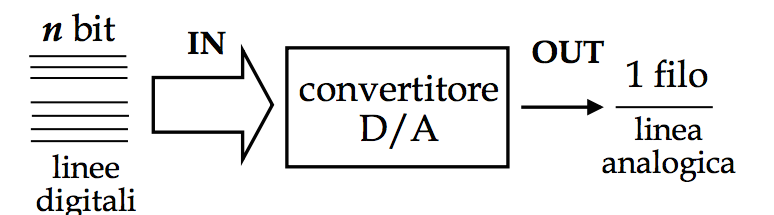
\includegraphics[scale=0.3]{cap3/dac}
    \caption{Schema di funzionamento di un convertitore Digitale-Analogico (DAC)}
    \label{dac}
  \end{center}
\end{figure}

\paragraph{Architetture DAC}
Esistono due architetture comuni di DAC:
\begin{enumerate}
	\item A resistori pesati (o \textit{Binary-weighted resistor})
	\item A scala R-2R (o \textit{R-2R resistor chain})
\end{enumerate}
\begin{figure}  
  \begin{center}
    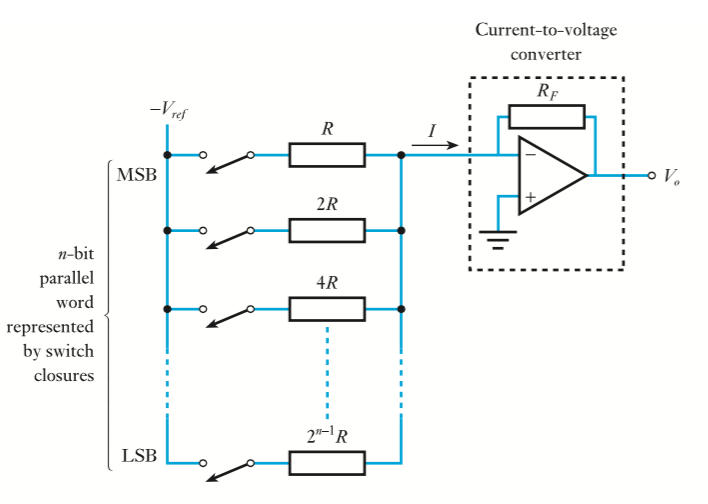
\includegraphics[scale=0.4]{cap3/bwdac}
    \caption{Struttura circuitale di un DAC a resistori pesati}
    \label{bwdac}
  \end{center}
\end{figure}
\subparagraph{\textbf{DAC a resistori pesati}} La Figura \ref{bwdac} illustra lo schema circuitale di un generico DAC a resistori pesati a n bit.
Il circuito, mostrato in figura, è costituito da $n$ interruttori pilotati dagli $n$ bit della parola in ingresso, $n$ resistori pesati su un valore di riferimento $R$, e un convertitore corrente-tensione invertente.

Ogni ingresso controlla un interruttore (\textit{switch}) che collega un resistore a un riferimento di tensione. Quando il generico bit dell'ingresso è a $1$ il corrispondente interruttore viene collegato al riferimento di tensione $-V_{ref}$, mentre quando il bit è a $0$ l'interruttore viene collegato a massa ($0 V$).

Data la corrente passante nell' $i$-esimo interruttore controllato dal bit $b_i$ della parola:
\begin{equation}
	I_i=-\frac{V_{ref}}{2^{(n-1)-i}R}b_i = -\frac{V_{ref}}{2^{(n-1)}R}2^ib_i
\end{equation}
si ricava la corrente complessiva della rete di resistori pesati:
\begin{equation}
	I = \sum_{k=1}^{n-1} I_k = -\frac{V_{ref}}{2^{(n-1)}R} \sum_{k=1}^{n-1} 2^k b_k 
\end{equation}
Infine, per effetto del convertitore corrente-tensione si ha:
\begin{equation}
	V_0 = -R_f I
\end{equation}
dove $R_f$ è il resistore di feedback. L'equazione definisce la relazione ingresso-uscita del DAC.

I vantaggi di questa configurazione sono la semplicità di realizzazione del circuito e l'utilizzo di un ristretto numero di resistenze ($n$ bit, $n$ resistenze). Per tale motivo le risoluzioni tipiche per questo metodo sono inferiori ai $10$ bit.

Lo svantaggio maggiore è la difficoltà nel realizzare resistenze con valori differenti e perfettamente calibrati, in modo tale che i loro rapporti tra esse siano precisi.
Per tale motivo questa configurazione è tuttavia poco usata nella pratica.

\subparagraph{\textbf{DAC a scala R-2R}}
Il DAC a resistenze pesate visto nella paragrafo precedente presenta problemi di realizzazione e di funzionamento, dovuti sostanzialmente all'uso di resistori molto differenti fra di loro. Questi problemi possono essere risolti usando un'altra architettura circuitale: il DAC a scala R-2R.

La figura \ref{r2rdac} illustra lo schema circuitale di un generico DAC a scala R-2R a $n$ bit.
Il circuito, mostrato in figura, è costituito da $n$ interruttori pilotati dagli $n$ bit della parola in ingresso, $n$ resistori e un convertitore corrente-tensione invertente. 

La differenza in questo caso è che tutti i resistori collegati agli interruttori hanno lo stesso valore $2R$. Inoltre, l'estremità di ogni resistore è collegata ad una catena di resistenze che va dall'ingresso invertente del convertitore corrente-tensione a massa.
\begin{figure}  
  \begin{center}
    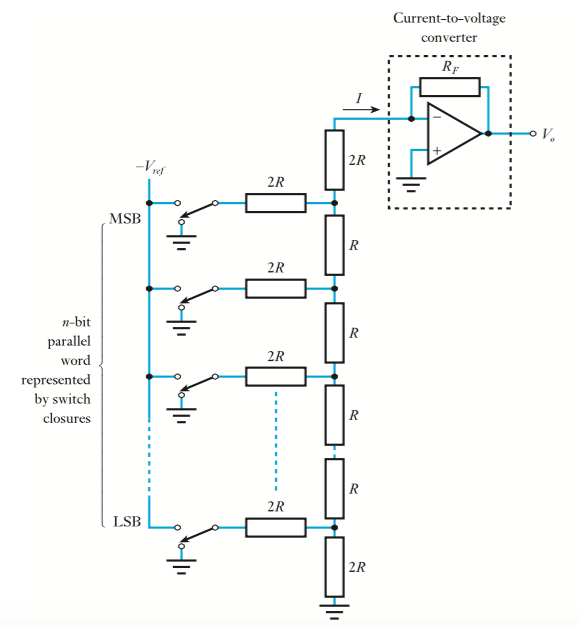
\includegraphics[scale=0.4]{cap3/r2rdac}
    \caption{Struttura circuitale di un DAC a scala R-2R}
    \label{r2rdac}
  \end{center}
\end{figure}

Il circuito è realizzato in modo tale che le correnti che fluiscono attraverso i resistori collegati agli interruttori vedano una resistenza $2R$ guardando in entrambe le direzioni lungo la catena delle resistenze. Pertanto, metà della corrente andrà in ciascuna direzione. 

Allo stesso modo, le correnti che scorrono lungo la catena vedono resistenze uguali in entrambe le direzioni e ad ogni nodo vengono nuovamente divise.

Riassumendo, ciascun interruttore contribuisce con metà della corrente fornita dall'interruttore sopra, e tale corrente viene ripetutamente dimezzata da ogni nodo incontrato nel percorso verso l'amplificatore operazionale.

Pertanto, le correnti generate dagli interruttori sono pesate, come nel metodo precedente, ma senza l'uso di un ampio intervallo di valori di resistenza. Dunque questa architettura presenta il vantaggio di utilizzare solo due valori resistivi risultando più facile da realizzare.

I tempi di conversione dei metodi precedentemente descritti sono simili. Essi sono determinati dal tempo impiegato dagli interruttori per cambiare stato e dal tempo di risposta dell'amplificatore operazionale. In generale il tempo di conversione cresce all'aumentare della risoluzione. Un DAC a $8$ bit per applicazioni generiche (\textit{general-purpose}) possiede tempi di conversione compresi tra i $100ns$ e $1ms$, mentre un convertitore a $16$ bit può avere un tempo di conversione nell'ordine dei microsecondi.

Per applicazioni specifiche, come nel caso del misuratore oggetto di questo lavoro di tesi, sono necessari convertitori ad alta velocità con tempi di conversione nell'ordine dei nanosecondi. Per raggiungere tali prestazioni l'uso di una singola architettura non basta, pertanto è necessario combinare due o più architetture allo scopo di raggiungere le prestazioni richieste. Il procedimento è noto come "segmentazione" e questa  architettura è chiamata "DAC segmentato” (\textit{Segmented DAC}). 

\paragraph{Convertitore DAC presente sulla scheda di conversione}
Il convertitore presente sulla scheda di conversione \textit{SCO Board} è il \textit{DAC902}. \'E un convertitore DAC Segmentato prodotto dalla \textit{Texas Instruments} con una risoluzione di $12$ bit e una velocità di campionamento massima pari a $165MHz$.
Tale architettura rispetta pienamente le specifiche prefissate con una frequenza di campionamento massima ben superiore a quella richiesta.

Questo convertitore utilizza la tecnica della somma di correnti vista nelle precedenti due architetture, ma al contrario di quest'ultime i generatori di corrente sono implementati con transistor PMOS invece che con resistori e tensioni di riferimento.
\begin{figure}  
  \begin{center}
    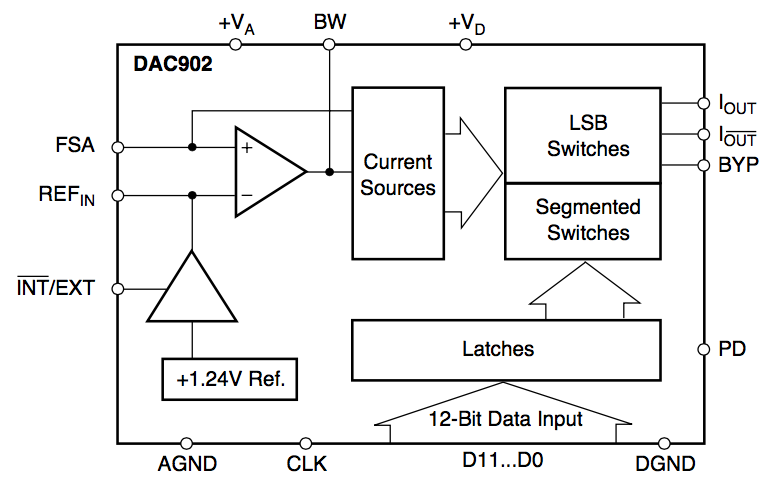
\includegraphics[scale=0.3]{cap3/schemadac902}
    \caption{Schema a Blocchi interno del DAC - DAC902}
    \label{schemadac902}
  \end{center}
\end{figure}
L'architettura segmentata utilizzata in questo integrato sfrutta due architetture: un DAC gestisce i bit più significativi (MSB) e un altro gestisce i bit meno significativi (LSB). Lo schema a blocchi è mostrato in figura \ref{schemadac902}.

Una descrizione più dettagliata dell'integrato è fornita sul sito del costruttore~\cite{sitedac902}.

\subsubsection{Convertitore ADC}
Il processo di campionamento di un segnale analogico consiste nel prelevare una lettura istantanea della sua grandezza e di convertirla in una forma digitale. Questa operazione è svolta dal convertitore Analogico-Digitale (ADC)~\cite{storeyelet}.
\begin{figure}  
  \begin{center}
    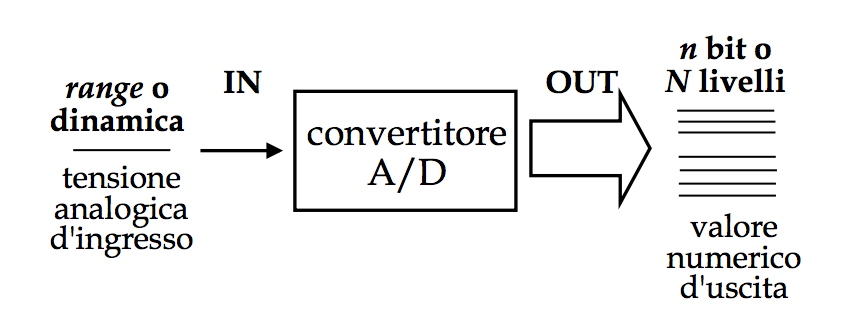
\includegraphics[scale=0.3]{cap3/adc}
    \caption{Schema di funzionamento di un convertitore Analogico-Digitale (ADC)}
    \label{adc}
  \end{center}
\end{figure}

\paragraph{Architetture ADC}
Esistono cinque architetture comuni di ADC:
\begin{enumerate}
	\item A conteggio (\textit{Counter})
	\item Ad approssimazioni successive (\textit{Successive Approximation})
	\item A Doppia rampa (\textit{Dual Slope})
	\item Flash
	\item Pipeline
\end{enumerate}

\subparagraph{\textbf{ADC a conteggio}}
\begin{figure}  
  \begin{center}
    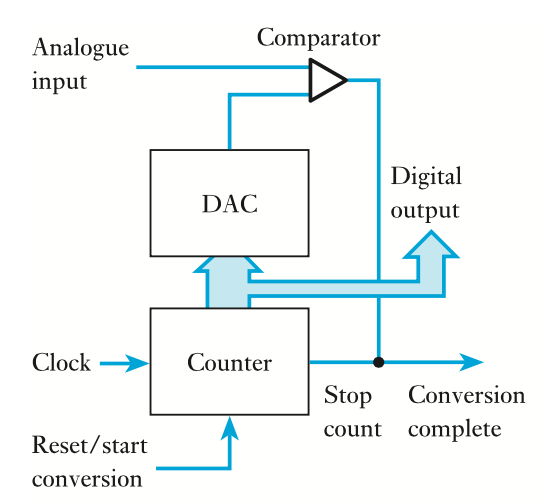
\includegraphics[scale=0.35]{cap3/adccounter}
    \caption{Schema di funzionamento di un ADC a conteggio}
    \label{adccounter}
  \end{center}
\end{figure}
L'ADC a conteggio è una delle forme più semplici di convertitore ADC. Lo schema di funzionamento è mostrato in Figura \ref{adccounter}.

Il cuore dell'architettura è costituito da un contatore incrementale. La conversione viene effettuata iniziando un nuovo conteggio a partire da zero. L'uscita del contatore viene convertita in analogico dal DAC e quindi confrontata con la tensione di ingresso mediante un comparatore. Un comparatore è un dispositivo che produce un'uscita booleana a seconda di quale dei due ingressi è maggiore. Quando il valore prodotto dal DAC supera la tensione di ingresso, il conteggio viene bloccato e tale valore rappresenta il valore di tensione di uscita.

Questo metodo è di semplice realizzazione, ma i principali difetti sono la lentezza e il tempo di conversione non costante. Per un ADC a $n$ bit, la conversione può richiedere nel caso pessimo $2^{n-1}$ cicli di clock. Il tempo di conversione è solitamente nell'ordine dei millisecondi (ca. $500 Sa/s$).

Una versione migliorata dell'ADC a conteggio è l'ADC a inseguimento (\textit{servo ADC}): il contatore incrementale viene sostituito con un contatore incrementale/decrementale. Pertanto, l'uscita del comparatore è utilizzata come segnale di comando del contatore, forzando il contatore a "inseguire" segnale di ingresso analogico. Esso risulta più veloce dell'ADC a conteggio, a condizione che i valori di tensione da convertire siano abbastanza vicini fra loro.

\subparagraph{\textbf{ADC ad approssimazioni successive}}
\begin{figure}  
  \begin{center}
    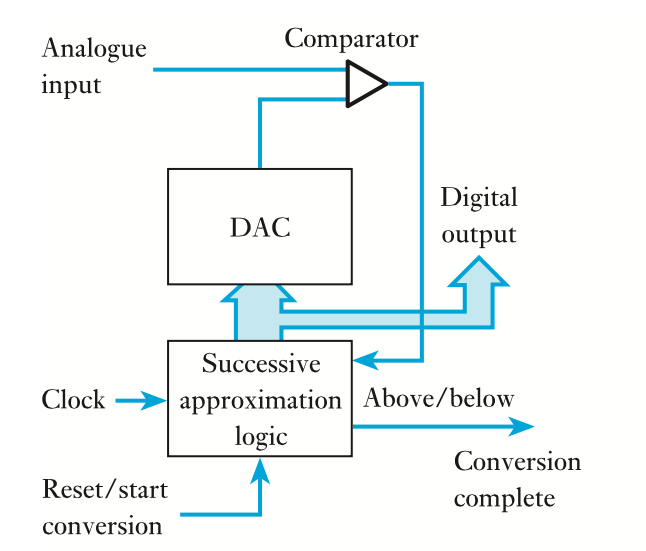
\includegraphics[scale=0.35]{cap3/adcsar}
    \caption{Schema di funzionamento di un ADC ad approssimazioni successive}
    \label{adcsar}
  \end{center}
\end{figure}
L'ADC ad approssimazioni successive è basato su una logica di controllo costituita da un registro ad approssimazioni successive chiamato SAR (\textit{Successive Approximation Register}). Lo schema di funzionamento è mostrato in Figura \ref{adcsar}.

Questa architettura è simile a quella dell'ADC a conteggio, fatta eccezione che il semplice contatore incrementale è sostituito dalla logica di controllo SAR. Come negli ADC a conteggio, la conversione avviene confrontando l'uscita di un convertitore DAC con la tensione in ingresso.

Il DAC viene comandato dalla parola digitale prodotta dalla logica di controllo. Inizialmente, tutti i bit della parola digitale sono impostati a 0 mentre il bit più significativo (MSB, \textit{Most Significant Bit}) è impostato a $1$. Questo valore viene convertito e confrontato con il segnale di ingresso analogico utilizzando il comparatore ed il risultato del comparatore viene inviato al SAR. Se la tensione di ingresso è maggiore della parola digitale corrente, il SAR mantiene l'MSB a 1 e carica un altro 1 nel bit immediatamente successivo, altrimenti pone l'MSB a 0 e carica sempre un 1 nel bit immediatamente successivo. I passi appena descritti vengono reiterati fino al bit meno significativo (LSB, \textit{Least Significant Bit}). Il metodo appena descritto è chiamato metodo di \textit{bisezione}.

Il tempo di conversione dell'ADC è costante qualunque sia il valore della tensione in ingresso. Indicando con $T_{ck}$ il periodo del clock e con $n$ bit il numero di bit del convertitore, il tempo di conversione $T_{conv}$ è pari a:
\begin{equation}
	T_{conv}=nT_{ck}
\end{equation}

Questa architettura raggiunge velocità di conversione migliori dell'ADC a conteggio, perdendo però in semplicità di realizzazione.

Solitamente i convertitori SAR possiedono risoluzioni comprese tra gli $8$ e i $12$ bit con tempi di conversione nell'ordine dei microsecondi ($50 \div 400 KSa/s$).

\subparagraph{\textbf{ADC a Doppia rampa}}
\begin{figure}  
  \begin{center}
    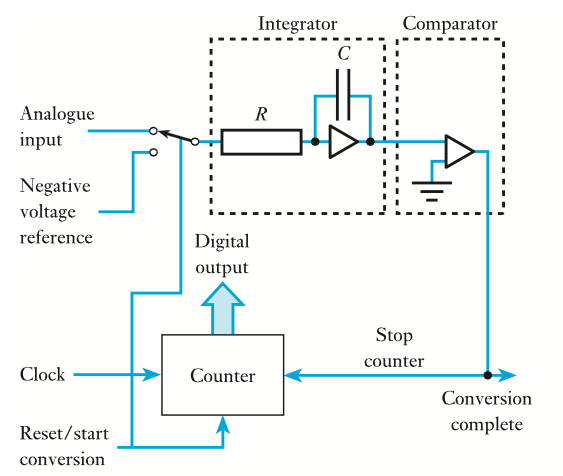
\includegraphics[scale=0.35]{cap3/adcdoppiarampa}
    \caption{Schema di funzionamento di un ADC a doppia rampa}
    \label{adcdoppiarampa}
  \end{center}
\end{figure}
L'ADC a doppia rampa è un convertitore basato sull'utilizzo di un integratore. Lo schema di funzionamento è mostrato in Figura \ref{adcdoppiarampa}.

L'amplificatore operazionale integra il segnale di ingresso per un determinato periodo di tempo, producendo una carica sul condensatore proporzionale alla tensione di ingresso. L'integratore viene poi collegato ad un riferimento di tensione negativo che permette di scaricare il condensatore ad una velocità costante.

Il tempo impiegato per scaricare il condensatore viene misurato da un contatore. Il tempo di scarica è proporzionale alla quantità di carica presente nel condensatore e quindi alla tensione di ingresso. Tale conteggio corrisponde al valore digitale prodotto in uscita.

Questa tecnica si utilizza in quelle applicazioni in cui il segnale da convertire varia lentamente nel tempo, privilegiando la precisione rispetto alla rapidità di conversione. Con questi convertitori è possibile raggiungere risoluzioni maggiori di $20$ bit portando però il tempo di conversione sull'ordine dei secondi ($10 \div 100 Sa/s$).

\subparagraph{\textbf{ADC Flash}}
\begin{figure}  
  \begin{center}
    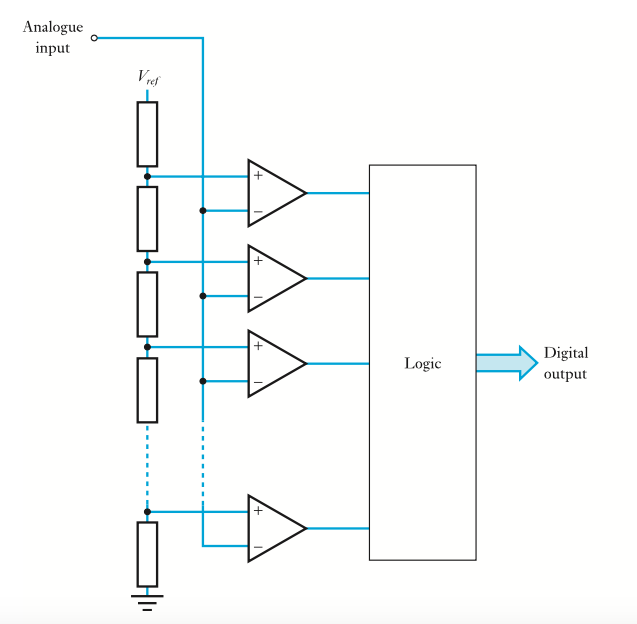
\includegraphics[scale=0.35]{cap3/adcflash}
    \caption{Schema di funzionamento di un ADC Flash}
    \label{adcflash}
  \end{center}
\end{figure}
L'ADC Flash è basato sull'utilizzo di compratori in parallelo. Lo schema di funzionamento è mostrato in Figura \ref{adcflash}.

Il segnale di ingresso di un ADC Flash a $n$ bit, viene confrontato con $2^n$ tensioni di riferimento, tipicamente generate con una stringa resistiva realizzata con $2^n$ resistori, tramite $2^n$ comparatori. Il risultato è che tutti i comparatori che hanno tensioni superiori alla tensione di ingresso produrranno un uscita di tensione positiva, mentre quelli collegati a tensioni al di sotto della tensione di ingresso produrranno tensioni di senso opposto. La logica combinatoria viene quindi utilizzata per determinare il valore digitale di uscita.

Il grosso vantaggio di questa tecnica è la velocità di conversione, essa permette di raggiungere tempi di conversione nell'ordine dei nanosecondi (fino a $40 GSa/s$): è la tecnica ADC più veloce. 

Lo svantaggio è l'alto costo di realizzazione ($n$ bit implica $2^n$ comparatori). Pertanto, le risoluzioni tipiche sono di $8$ bit.

\subparagraph{\textbf{ADC Pipeline}}
\begin{figure}  
  \begin{center}
    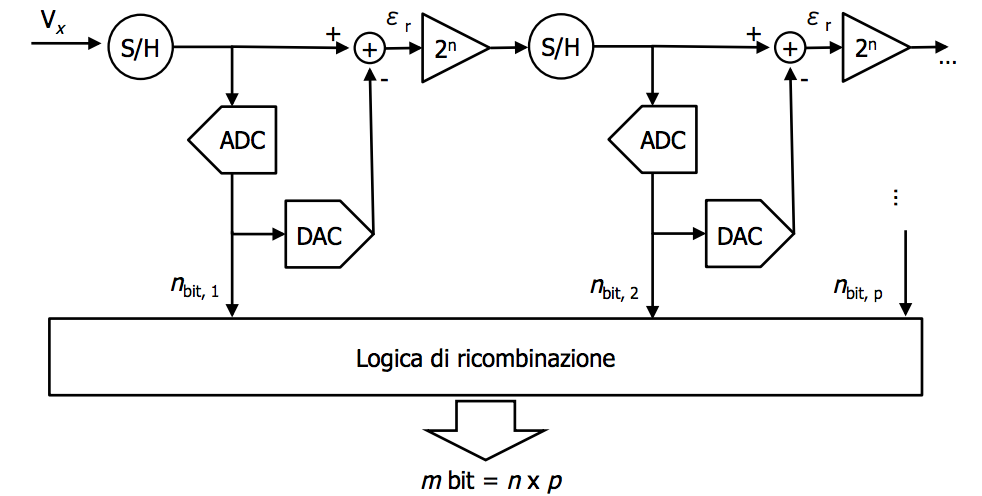
\includegraphics[scale=0.3]{cap3/adcpipeline}
    \caption{Schema di funzionamento di un ADC Pipeline }
    \label{adcpipeline}
  \end{center}
\end{figure}
L'ADC Pipeline è un convertitore che sfrutta il principio della pipeline. Lo schema di funzionamento è mostrato in Figura \ref{adcpipeline}.

Una pipeline è un insieme di stadi di elaborazione connessi in serie, in cui l'uscita di un elemento è l'ingresso del successivo. Gli stadi sono identici, quindi è sufficiente spiegare il funzionamento del primo per comprendere il funzionamento di tutta l'architettura.

Il segnale analogico d'ingresso viene convertito da un ADC SAR a $n$ bit. Il segnale digitale così prodotto costituisce l'uscita dello stadio. Il segnale ottenuto dal SAR, oltre che essere l'uscita dello stadio, costituisce l'ingresso di un DAC, che fornisce in uscita nuovamente un segnale analogico, che però differisce da quello originale in quanto affetto da errore di quantizzazione introdotto dal SAR.

Il campione così ottenuto va in ingresso a un sommatore che ne fa la differenza col segnale analogico originale, ottenendo così come risultato l'errore di quantizzazione. Successivamente l'errore di quantizzazione va in ingresso a un amplificatore di guadagno $2^n$, in modo da poter sfruttare al massimo l'intervallo di conversione del ADC SAR. Infine, gli stadi successivi al primo convertono l'errore di quantizzazione. I bit ottenuti in uscita dai diversi stadi vengono poi riallineati tramite opportuni registri, in modo da costituire la parola digitale di uscita. 

La risoluzione di un convertitore Pipeline risulta limitata dalla precisione dei convertitori AD e DA presenti nell'architettura. La massima risoluzione ottenibile si aggira da un minimo di $8$ bit a un massimo di $24$ bit  con velocità di conversione sull'ordine dei nanosecondi ($1 \div 200 MSa/s$). 

\paragraph{Convertitore ADC presente sulla scheda di conversione}
Il convertitore presente sulla scheda di conversione \textit{SCO Board} è l'\textit{ADS807}. \'E un convertitore ADC Pipeline prodotto dalla \textit{Texas Instruments} con una risoluzione di $12$ bit e una velocità di campionamento massima pari a $53MHz$. Tale convertitore rispetta pienamente le specifiche prefissate.

\begin{figure}  
  \begin{center}
    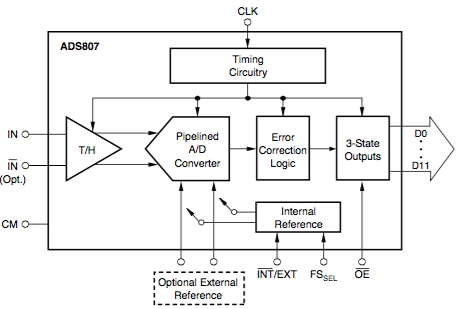
\includegraphics[scale=0.5]{cap3/ads807schema}
    \caption{Schema di funzionamento del ADS807}
    \label{ads807schema}
  \end{center}
\end{figure}

La figura \ref{ads807schema} mostra lo schema a blocchi interno del \textit{ADS807}.
Il circuito è costituito da quattro componenti principali:
\begin{itemize}
	\item \underline{Circuito di Track \& Hold}: L'ingresso analogico consiste in un circuito differenziale di \textit{Track \& Hold}. Tale circuito è utilizzato per mantenere il segnale campionato costante durante tutto il periodo di conversione. A differenza di un \textit{Sample \& Hold}, il \textit{Track \& Hold} trascorre la maggior parte del tempo seguendo l'ingresso ed è posto in modo hold solo per un breve intervallo. Nei sistemi di acquisizione che operano ad elevate velocità, come in questo caso (superiori a $1MHz$), i termini \textit{Sample \& Hold} e \textit{Track \& Hold} perdono la loro distinzione.
	\item \underline{ADC Pipeline}: L'architettura a Pipeline è formata da $12$ stadi interni con una latenza di $6$ cicli di clock. I dati in uscita diventano validi sul fronte di salita del clock.
	\item \underline{Logica per la correzione dell'errore (Error Correction Logic)}: La logica di correzione dell'errore è quella descritta nel paragrafo precedente dove il campione digitale prodotto ogni stadio della pipeline viene convertito da un DAC e sottratto al valore analogico di ingresso producendo così un errore di quantizzazione che verrà amplificato e inviato allo stadio successivo.
	\item \underline{3 State Outputs}: L'uscita digitale del convertitore possiede una logica a $3$ stati. Nella logica \textit{tri-state} è presente un terzo stato, detto ad alta impedenza, oltre ai due livelli logici già presenti nella logica binaria. Nello stato ad alta impedenza l'uscita si comporta come se fosse elettricamente disconnessa dal resto del circuito.
\end{itemize}
Una descrizione più dettagliata dell'integrato è fornita sul sito del produttore~\cite{siteads807}.

\section{Parte digitale}
La parte digitale dello strumento è composta da una scheda \textit{embedded} di prototipazione. 

\subsection{Scheda di prototipazione utilizzata}
\begin{figure}  
  \begin{center}
    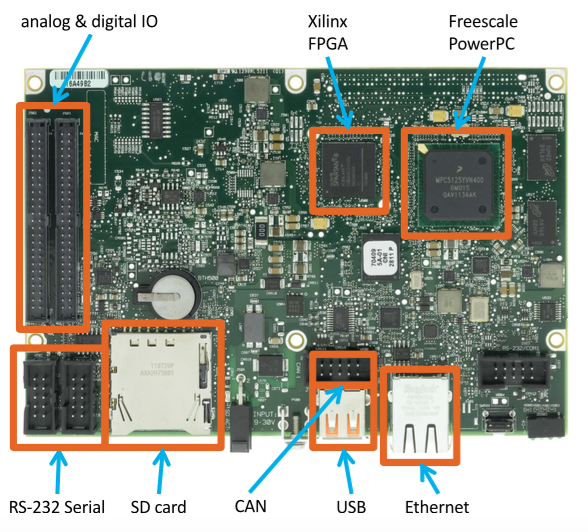
\includegraphics[scale=0.4]{cap3/sbrio}
    \caption{Scheda di elaborazione digitale, National Instruments Single-Board RIO (sbRIO) 9636}
    \label{sbrio}
  \end{center}
\end{figure}
Per lo svolgimento della fase di prototipazione dello strumento è stata utilizzata la scheda di prototipazione \textit{Single Board RIO 9636}, progettata e prodotta dalla \textit{National Instruments}, Figura \ref{sbrio}.

La principale motivazione che ha spinto all'utilizzo di un dispositivo \textit{embedded} di prototipazione è la possibilità di raggiungere elevate prestazioni di calcolo. Inoltre, l'estrema ri-configurabilità di tale dispositivo ha permesso una rapida prototipazione dello strumento.

La scheda integra su un singolo PCB molteplici componenti elettronici; sono infatti presenti un microprocessore, in grado di eseguire software \textit{Real-Time}, una FPGA, \textit{Xilinx Spartan-6 LX45}, un DAC ed un ADC. Inoltre la scheda integra $4$ output e $16$ input analogici, a $16$-bit, e $28$ canali digitali, programmabili per essere utilizzati come input o output.

Sono presenti infine un connettore \textit{10/100Base-T Ethernet} per la comunicazione con un PC, una USB, un lettore di SDHC, un connettore CAN e due connettori seriali (RS232 e RS485). Delle numerose componenti presenti sulla scheda, per il progetto presentato in questa tesi sono stati sfruttati, oltre al microprocessore ed all'FPGA, soltanto la connessione \textit{Ethernet}, per comunicare con un PC host, e $24$ dei $28$ pin digitali ($12$ in ingresso e $12$ in uscita) per la comunicazione con i convertitori della scheda di conversione \textit{SCO Board}.

A causa dei vincoli stringenti sulla temporizzazione non è stato possibile sfruttare i convertitori integrati nella \textit{sbRIO}, che sono stati sostituiti con i componenti precedentemente descritti. Una descrizione più dettagliata della scheda è fornita sul sito di \textit{National Instruments}~\cite{sitesbrio}.

Poiché la parte centrale dell'architettura software è stata sviluppata per essere eseguita da un'FPGA, in questo capitolo si darà ampio spazio ad una spiegazione generale della nascita e delle principali tecnologie impiegate nella costruzione di FPGA.

\subsection{FPGA}
Con il termine FPGA, acronimo di \textit{Field Programmable Gate Array}, si intende un circuito integrato le cui funzionalità sono programmabili via software~\cite{Kuon:2008:FAS:1454695.1454696}. Rispetto ad una soluzione specializzata (ASIC, ovvero \textit{Application Specific Integrated Circuit}) offrono numerosi vantaggi, infatti per la realizzazione di un'ASIC possono trascorrere mesi e la spesa è dell'ordine di centinaia di migliaia di dollari solo per la realizzazione del primo prototipo; al contrario un'FPGA può essere riconfigurata in pochi secondi e i suoi costi non superano qualche migliaio di dollari.

I vantaggi in termini di costo e velocità di sviluppo sono compensati da una maggiore area occupata, tipicamente dalle $20$ alle $35$ volte, una computazione $3$-$4$ volte più lenta e un consumo energetico circa $10$ volte maggiore~\cite{4068926}.

Nonostante questi svantaggi le FPGA sono preferite in ambiti in cui i volumi di produzione non sono tali da giustificare la spesa per la realizzazione di un ASIC, e spesso rappresentano l'unica alternativa economicamente sostenibile.

\subsubsection{Storia delle FPGA}
L'origine delle moderne FPGA può essere ricondotta allo sviluppo dei circuiti integrati negli anni $'60$. 

I primi dispositivi programmabili avevano architetture regolari e funzionalità flessibili. Infatti tipicamente si avevano architetture composte da array bidimensionali di porte logiche, con connessioni punto-punto, detti \textit{cellular array}.

Questi primi array contenevano celle logiche che potevano essere programmate, attraverso la "metallizzazione", durante il processo produttivo per creare funzioni logiche a due ingressi. A metà degli anni $'60$ si è raggiunta la capacità di programmare i circuiti sul campo, ovvero dopo il processo di produzione, attraverso l'introduzione di "punti di taglio"~\cite{Minnick:1967:SMR:321386.321387} nei \textit{cellular array}. Le connessioni tra i diversi elementi logici erano ancora fisse, ma la funzionalità di ogni cella logica era modificabile grazie all'introduzione di fusibili programmabili. Questi fusibili erano programmabili sul campo attraverso l'uso di correnti di programmazione.

Negli anni $'70$ sono state introdotte le memorie PROM, che hanno portato nuovi modi di implementare funzioni logiche. Nonostante una ROM a $N$ indirizzi possa implementare qualsiasi funzione logica con $N$ ingressi, l'efficienza rispetto all'area si rivela essere un problema. Infatti l'area dipende in modo esponenziale dal numero di ingressi $N$ e quindi, anche con valori piccoli di $N$, il chip avrà dimensioni elevate.

\begin{figure}
\centering
\subfigure[PLA]
{\label{plasa}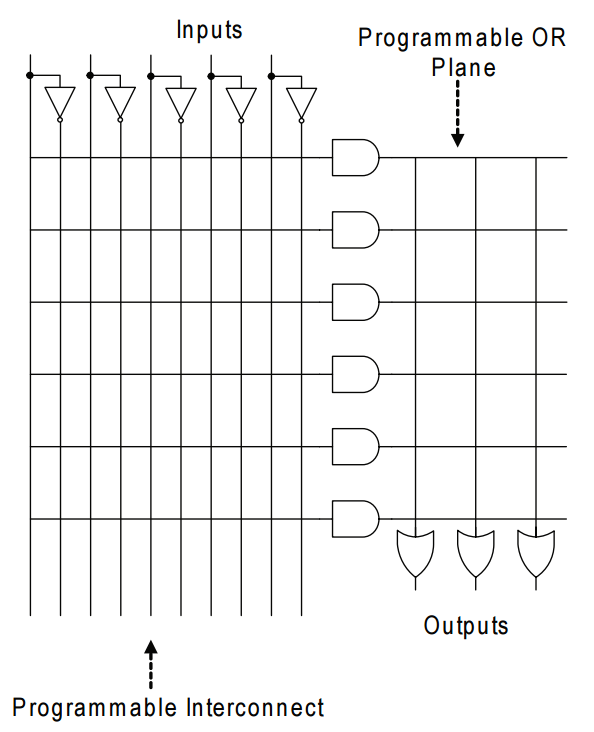
\includegraphics[scale=.3]{cap3/pla}}
\hspace{5mm}
\subfigure[PLA con piano OR fisso]
{\label{plasb}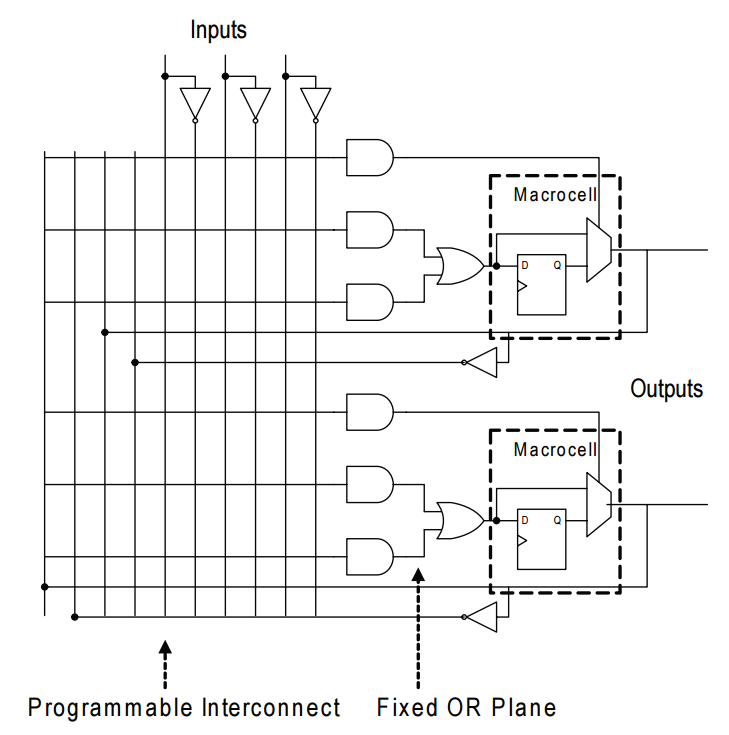
\includegraphics[scale=.3]{cap3/plaor}}
\caption{Tipologie di PLA}\label{plas}
\end{figure}

I primi dispositivi programmabili, chiamati PLA (\textit{Programmable Logic Array}) si basavano su questa architettura, con una struttura a due livelli, AND e OR. Un esempio di PLA è mostrato in Figura \ref{plasa}.

Questa architettura si è poi evoluta in un piano AND programmabile, seguito da un piano OR fisso (Figura \ref{plasb}). Questa seconda architettura mantiene comunque una buona flessibilità, ma al tempo stesso riduce la complessità del circuito.

Quest'architettura è stata introdotta sul mercato nel $1977$ da \textit{Monolithic Memories Incorporated} (MMI)~\cite{birkner1978programmable}.

Per realizzare una funzione logica con questo tipo di architettura è necessario usare uno o due livelli della struttura. Gli input e le combinazioni intermedie alimentano l'array attraverso un'interconnessione programmabile, tipicamente una \textit{crossbar}. Questo tipo di implementazione dell'interconnessione porta ad una crescita dell'area molto rapida, soprattutto per circuiti con molti ingressi.

La prima memoria basata su FPGA (\textit{SRAM-based FPGA}) è stata introdotta da \textit{Wahlstrom} nel $1967$~\cite{wahl}. 

Questa architettura usa uno stream di bits sia per la logica che per l'interconnessione. Al contrario della \textit{cellular array} ogni cella logica può implementare sia una funzione logica che una memoria. Inoltre, la connessione tra celle logiche può essere facilmente modificata per permettere l'implementazione di diverse topologie del circuito. Nonostante la memoria statica (SRAM) offra una flessibilità maggiore nella programmabilità, richiede un'area maggiore rispetto all'implementazione ROM.

Questo problema ha ritardato l'introduzione in commercio di prodotti basati su memoria statica fino alla metà degli anni $'80$, quando il costo per transistor era diventato sufficientemente basso.

La prima FPGA moderna è stata introdotta da \textit{Xilinx} nel $1984$~\cite{reconfgate}, e conteneva la classica configurazione ad array di elementi logici configurabili. In particolare era formata da $64$ blocchi logici e $58$ input e output. 

Dal primo esempio commerciale le FPGA sono cresciute enormemente, infatti una moderna FPGA può contenere oltre $300000$ elementi logici equivalenti, ed oltre $1000$ input ed output, in aggiunta ad elementi logici specializzati, che hanno permesso alle FPGA di incrementare le loro funzionalità e quindi le loro possibili applicazioni.

\subsubsection{Tecniche di implementazione delle FPGA}
Come già accennato in precedenza, una FPGA consiste in un array di blocchi logici programmabili, potenzialmente di tipo differente, che includono logica generica, celle di memoria e moltiplicatori, circondati da una rete di routing programmabile, che permette di modificare l'interconnessione via software.

\begin{figure}  
  \begin{center}
    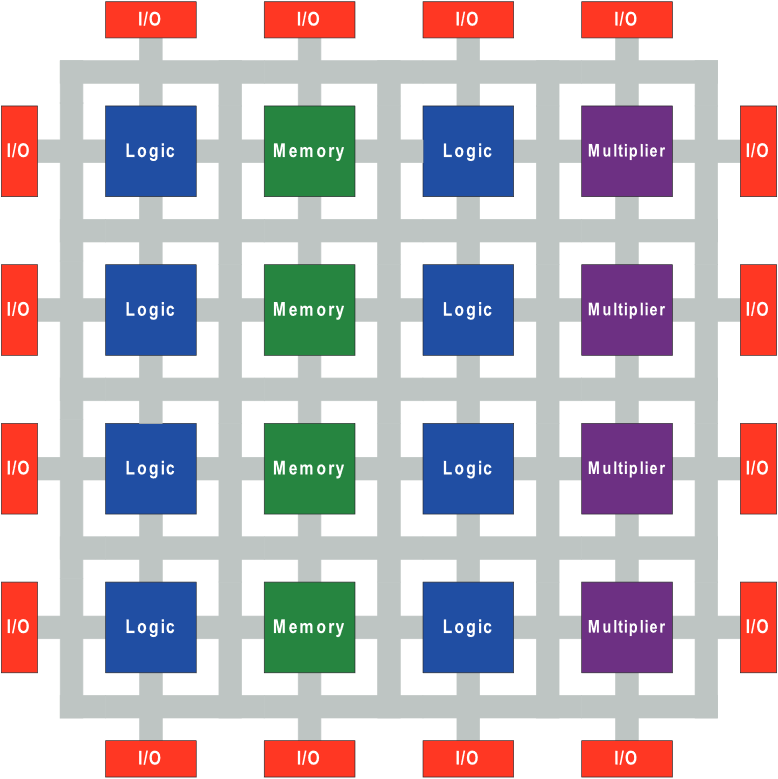
\includegraphics[scale=0.3]{cap3/chipFPGA}
    \caption{Struttura semplificata del chip FPGA}
    \label{chipFPGA}
  \end{center}
\end{figure}
L'array è circondato da una serie di blocchi input/output programmabili, che connettono il chip con il mondo esterno. La struttura semplificata del chip è presentata in Figura \ref{chipFPGA}.

Ogni FPGA si affida alla presenza di switch programmabili, che sono usati per dare al chip la sua caratteristica di programmabilità.

Nel corso degli anni sono state introdotte diverse tecniche per rendere programmabile un chip, partendo dalle EPROM, EEPROM, per arrivare alle tecniche  \textit{static-memory}, \textit{flash} ed \textit{anti-fuse}.

Di tutte le tecnologie introdotte soltanto le ultime $3$ sono attualmente implementate nei moderni prodotti commerciali. In seguito saranno trattate soltanto le tecnologie attualmente in uso.

\paragraph{Static-memory}
\begin{figure}
\centering
\subfigure[Static Memory Cell]
{\label{staticmema}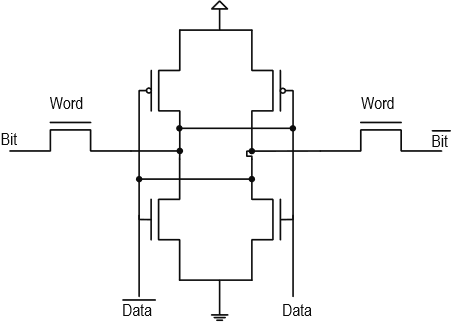
\includegraphics[scale=.35]{cap3/sma}}
\hspace{5mm}
\subfigure[Multiplexer con Static Memory Cell]
{\label{staticmemb}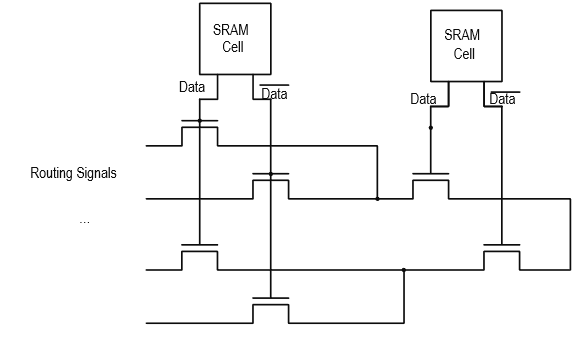
\includegraphics[scale=.35]{cap3/smb}}
\hspace{5mm}
\subfigure[Static Memory Cell e Lookup Table]
{\label{staticmemc}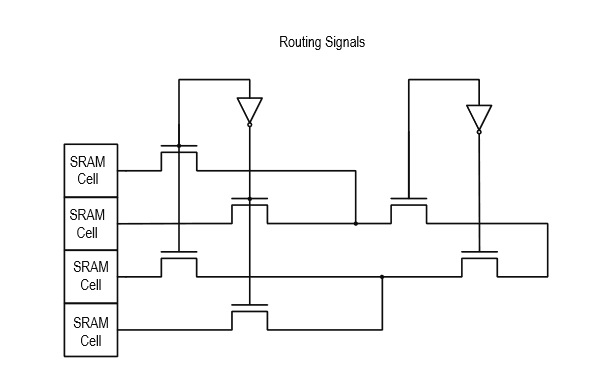
\includegraphics[scale=.35]{cap3/smc}}
\caption{Static Memory}\label{staticmem}
\end{figure}
Le celle statiche di memoria sono la base per la tecnologia SRAM. In questi dispositivi, le celle di memoria statica (Figura \ref{staticmema}) sono distribuite all'interno del chip FPGA, per garantire la programmabilità.

In questo tipo di architettura le SRAM hanno due principali utilizzi; alcune celle di memoria svolgono la funzione di \textit{multiplexer}, per guidare i segnali attraverso le interconnessioni, mentre la maggior parte delle celle implementano le \textit{Look Up Table} (LUT), che sono utilizzate tipicamente per implementare funzioni logiche. Le Figure \ref{staticmemb} ed \ref{staticmemc} illustrano questi possibili utilizzi.

La tecnologia SRAM è la più utilizzata nell'industria di FPGA per due principali vantaggi che porta, l'uso del processo produttivo CMOS standard e la riprogrammabilità. Una cella di memoria SRAM può essere riprogrammata un numero illimitato di volte. Un circuito dedicato presente nel chip inizializza tutti i bit delle SRAM all'avvio, sulla base di una configurazione fornita dall'utente.

A differenza delle altre tecnologie, l'uso di SRAM non richiede particolari lavorazioni sul circuito integrato, ma, come già detto, permette l'uso della tecnica CMOS standard. Questo porta come conseguenza diretta la possibilità di beneficiare dell'aumento di concentrazione di transistor, velocità e consumo energetico portati dell'uso del più recente processo produttivo disponibile sul mercato.

Tuttavia l'uso della tecnologia SRAM porta ad un certo numero di svantaggi:
\begin{itemize}
	\item \underline{Area}: Una cella SRAM richiede $5$-$6$ transistor, e l'elemento riprogrammabile usato per indirizzare i segnali richiede un transistor aggiuntivo.
	\item \underline{Volatilità}: Le celle di SRAM sono volatili; ciò significa che è necessario usare un dispositivo esterno per salvare la configurazione in modo permanente quando il dispositivo è spento. Questi dispositivi di memoria portano ad un'incremento di costo nell'FPGA.
	\item \underline{Sicurezza}: \'E possibile che la configurazione sia intercettata e rubata, a causa della necessità di caricare il contenuto delle SRAM all'avvio del dispositivo.
	\item \underline{Proprietà elettriche dei transistor di passaggio}: Le FPGA basate su SRAM utilizzano transistor di passaggio per implementare i multiplexer. Tuttavia questi transistor non possono essere considerati switch ideali, poiché hanno una resistenza ed una capacità non trascurabili, che possono portare a problemi nell'uso di processi produttivi piccoli.
\end{itemize}

\paragraph{Flash/EEPROM}
Una tecnologia per superare alcuni degli svantaggi presenti nella tecnologia SRAM è basata sull'uso di transistor con tecnologia \textit{floating gate}. 

Questo approccio sta alla base dell'implementazione delle celle di memoria flash ed EEPROM. Queste celle di memoria hanno la caratteristica di non essere volatili, quindi i dispositivi basati su questa architettura non hanno necessità di salvare la configurazione fornita dall'utente in memorie separate.

Storicamente le EEPROM non erano usate per controllare gli switch sui segnali dell'FPGA, ma erano usate per implementare le funzioni AND nei dispositivi PLD~\cite{fpgabook}. Questa tecnica non è più usata, tranne che nei dispositivi a piccola capacità~\cite{cpldxilinx}, a causa dell'eccessivo consumo statico dei dispositivi con questa architettura.

I moderni processi produttivi hanno permesso di utilizzare le celle di memoria \textit{floating gate} direttamente come switch. In particolare attualmente sono usate celle di memoria flash a causa della loro efficenza rispetto all'area. L'uso diffuso di memorie flash come memoria non volatile del chip assicura vantaggi nella diminuzione della dimensione geometrica dei transistor.

\begin{figure}  
  \begin{center}
    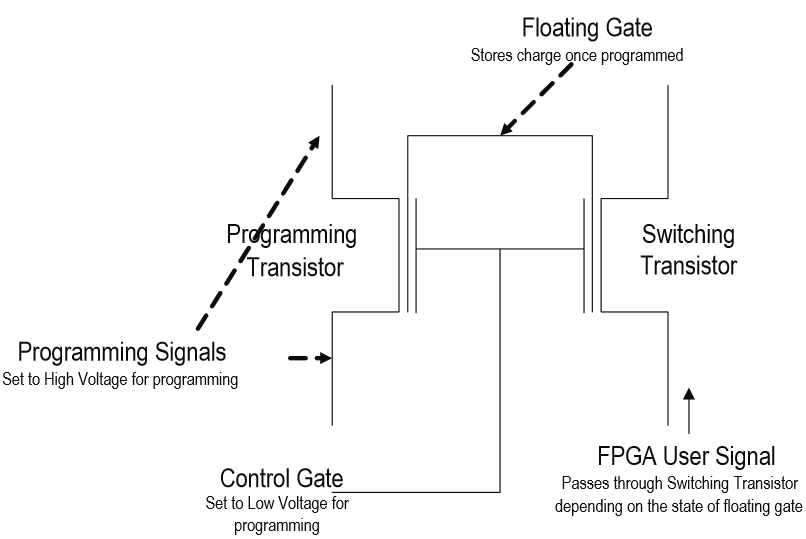
\includegraphics[scale=0.4]{cap3/floatgate}
    \caption{Implementazione del floating gate}
    \label{floatgate}
  \end{center}
\end{figure}

La Figura \ref{floatgate} mostra l'implementazione del \textit{floating gate} nei dispositivi della linea \textit{ProASIC} di \textit{Actel}~\cite{actelpro}. 

Il transistor più piccolo, nella Figura \ref{floatgate} \textit{programming transistor}, è usato per programmare il \textit{floating gate}, iniettando carica che rimane anche quando il dispositivo è spento, mentre il transistor più grande, nella figura \textit{switching transistor}, funge da switch programmabile. Questa implementazione basata su memoria flash offre molteplici vantaggi, il più importante è la non volatilità. Inoltre, a causa della non volatilità, un dispositivo flash funzionerà immediatamente all'accensione, non dovendo aspettare il caricamento della configurazione.

Tuttavia la logica di programmazione introduce un overhead in area non presente nell'implementazione SRAM; questo costo è comunque modesto ed è ammortizzabile su un gran numero di elementi programmabili.

Paragonata alla tecnologia \textit{anti-fuse}, un'architettura non volatile alternativa che verrà approfondita nel paragrafo successivo, i dispositivi flash hanno il vantaggio di essere riconfigurabili e di poter essere programmati senza essere rimossi dal circuito stampato.

L'uso dei transistor \textit{floating gate} richiede una particolare attenzione nella fase di progettazione, per assicurare che la tensione \textit{source-drain} rimanga sufficientemente bassa da prevenire iniezione di carica nel \textit{floating gate}~\cite{510550}. Tuttavia, con l'uso di processi produttivi sempre più piccoli, e di conseguenza tensioni sempre meno elevate, questo problema perde di importanza.

I principali svantaggi dell'architettura flash sono l'impossibilità di riprogrammare il dispositivo un numero infinito di volte. La carica presente nello strato di ossido ad un certo punto non permette più di cancellare e riprogrammare il dispositivo correttamente~\cite{622505}. I dispositivi attuali permettono di essere riprogrammati fino a $500$ volte, un numero che nella maggior parte dei casi si rivela sufficiente.

Un altro svantaggio della tecnologia flash è l'uso di un processo CMOS non standard. Infine, come già spiegato per l'architettura SRAM, anche l'architettura flash soffre della presenza di resistenze e capacità non trascurabili causate dall'uso di transistor come switch. Un trend che sta emergendo ultimamente è l'uso di memorie flash in combinazione con tecnologie riconfigurabili SRAM. In alcuni dispositivi prodotti da \textit{Altera}, \textit{Xilinx} e \textit{Lattice} la memoria flash è usata per garantire la non volatilità, mentre la SRAM fornisce la riprogrammabilità. Questo tipo di dispositivi, da un punto di vista architetturale, non sono diversi dai puramente SRAM.

Rispetto ad un dispositivo puramente SRAM si guadagna quindi la non volatilità, ma si va a perdere il vantaggio nell'uso di un  processo produttivo standard e si introduce un overhead in termini di area a causa della replicazione dei bit, salvati sia in memorie flash che SRAM.

\paragraph{Anti-fuse}
Una tecnologia alternativa a SRAM e ai transistor \textit{floating gate} è la tecnologia programmabile \textit{anti-fuse}. Le interconnessioni di questa tecnologia sono strutture che in circostanze nominali mostrano una resistenza molto alta, ma che possono essere programmaticamente connessi per creare canali a bassa resistenza. A differenza delle precedenti tecniche, il collegamento è permanente. L'elemento programmabile, detto \textit{anti-fuse}, è usato direttamente per trasmettere i segnali all'interno dell'FPGA.

Per implementare gli anti-fuse sono usati due approcci:
\begin{enumerate}
	\item \underline{Dielettrico}: Gli anti-fuse dielettrici sono composti da un dielettrico posizionato tra lo strato $N+$ e il polisilicio \cite{32929}. L'applicazione di alte tensioni causano la rottura del dielettrico e formano un link conduttore con una resistenza tipicamente tra i $100$ e i $600\Omega$ \cite{231343}.
	\item \underline{Metal-to-metal}: Gli anti-fuse \textit{metal-to-metal} hanno largamente sostituito l'implementazione dielettrica. Questi \textit{anti-fuse} sono formati da due strati di metallo, separati da uno strato di isolante (tipicamente silicio amorfo o ossido di silicio). Anche in questo caso l'applicazione di alte tensioni causa la rottura dell'\textit{anti-fuse} e lo rende conduttivo. Il vantaggio di questa implementazione è la resistenza molto più bassa, tipicamente tra i $20$ e i $100 \Omega$ \cite{584227}.
\end{enumerate}

Il principale vantaggio della tecnologia \textit{anti-fuse} è il basso utilizzo di area. In particolare, con l'implementazione \textit{metal-to-metal}, non è richiesta area in silicio per creare le connessioni; ciò diminuisce l'overhead in termini di area causato dalla programmabilità. Tuttavia questo decremento in termini di area è compensato dalla necessità di introdurre transistor di programmazione molto grandi, che devono fornire correnti elevati per programmare gli \textit{anti-fuse}. Anche se questa area può essere distribuita tra molti \textit{anti-fuse} con una progettazione opportuna, gli \textit{anti-fuse} hanno un vantaggio aggiuntivo: hanno resistenze e capacità parassite più basse rispetto alle altre tecnologie.

L'area minore, la capacità e la resistenza ridotte permettono di includere più switch per dispositivo che nelle altre tecnologie. La non volatilità, come per i dispositivi basati su flash, significa che il dispositivo è pronto all'uso all'accensione; questo abbassa i costi, poiché non è necessaria una memoria aggiuntiva, e rende la tecnologia utilizzabile in quegli ambiti in cui il dispositivo deve essere pronto all'uso una volta acceso. Dato che la programmazione dell'FPGA va fatta una sola volta è possibile eseguirla in un ambiente controllato, migliorando così la sicurezza nel design dell'FPGA. Attualmente anche le altre tipologie di programmazione forniscono una modalità sicura, che disabilita l'accesso all'interfaccia di programmazione una volta che il dispositivo è programmato.

La tecnologia \textit{anti-fuse} porta anche notevoli svantaggi. In particolare, l'uso di un processo CMOS non standard comporta l'uso di processi produttivi molto meno all'avanguardia rispetto all'architettura SRAM. Inoltre, la tecnica adottata per la programmazione, che implica cambiamenti significativi nelle proprietà dell'\textit{anti-fuse}, porta a problemi di scaling. La tecnologia \textit{anti-fuse} più avanzata (nel $2005$) utilizza processi produttivi a $150nm$ \cite{axfpga}, che è diverse generazioni indietro rispetto alle più moderne tecnologie CMOS ($90nm$ nel $2004$ e $65nm$ nel $2006$).

L'impossibilità di riprogrammazione rende inutilizzabile questo tipo di dispositivi in ambiti dove sono necessari cambiamenti di configurazione, ma li rende ideali in ambiti in cui il rischio di corruzione delle memorie è elevato, come ad esempio l'ambito delle esplorazioni spaziali.

A differenza delle altre tecnologie, per l'\textit{anti-fuse} non è possibile la programmazione su circuito stampato. Al contrario è necessario utilizzare specifici dispositivi di programmazione per programmare il chip prima che sia montato sul prodotto finito.

Infine la caratteristica di singola programmazione non consente ai produttori di testare gli \textit{anti-fuse} per individuare possibili errori di produzione. Alcuni difetti possono essere individuati solo dopo la programmazione.

\subsection{Xilinx Spartan-6 LX45}
L'FPGA integrata nella scheda di prototipazione usata è la \textit{Spartan-6 LX45}, prodotta da \textit{Xilinx}.

In particolare questo prodotto integra al suo interno $54576$ registri \textit{Flip Flop} e 27288 \textit{Look Up Table} (LUT) a 6 ingressi raggruppati in $6822$ \textit{Slices} (blocchi logici che contengono 8 Flip Flop e 4 LUT). Inoltre sono integrati $58$ \textit{DSP48} (che contengono un moltiplicatore $18x18$ , un sommatore ed un accumulatore), $5$ canali DMA, $2088$ Kbits di block RAM e $358$ moduli di input/output riconfigurabili. 

La scheda possiede un'oscillatore a $40MHz$, da cui possono essere derivati clock in un intervallo compreso tra $2.5MHz$ e $320MHz$. La tecnologia usata per implementare lo switching è SRAM. 

Una descrizione più dettagliata dell'FPGA utilizzata può essere trovata nella documentazione fornita da \textit{Xilinx}\cite{dsxilinx}.

\subsubsection{Utilizzo area FPGA}
Il codice sviluppato per lo strumento di misura descritto in questo elaborato ha portato ad un notevole utilizzo di area del FPGA. I valori di utilizzo sono riportati in tabella \ref{tabarea}. Inoltre, sono stati sfruttati due diversi clock di frequenza $30MHz$ e $60MHz$.

\begin{table}[ht]
\centering
\begin{tabular}{l|l|l|l}
                                        & \textbf{Utilizzati} & \textbf{Totali} & \textbf{Utilizzo {[}\%{]}} \\ \hline
\textbf{Slices}                         & 5560                & 6822            & 81,5                                      \\
\textbf{Registri (FF)}                  & 13465               & 54576           & 24,7                                      \\
\textbf{Look Up Table (LUT)}            & 18003               & 27288           & 66                                        \\
\textbf{Block RAM}                      & 57                  & 116             & 49,1                                      \\
\textbf{Digital Signal Processor (DSP)} & 57                  & 58              & 98,3                                      \\
\textbf{DMA Channel}                    & 5                   & 5               & 100                                      
\end{tabular}
\caption{Valori di utilizzo di area dell'FPGA}
\label{tabarea}
\end{table}

\subsection{Microcontrollore}
Un microcontrollore è un dispositivo elettronico integrato in un singolo chip, utilizzato in alternativa ad un microprocessore nei sistemi \textit{embedded}, ed in particolare per applicazioni specifiche di controllo digitale.

Il microcontrollore utilizzato per il progetto descritto in questo elaborato, codice prodotto \textit{MPC5125}, è prodotto da \textit{Freescale}. 

\begin{figure}  
  \begin{center}
    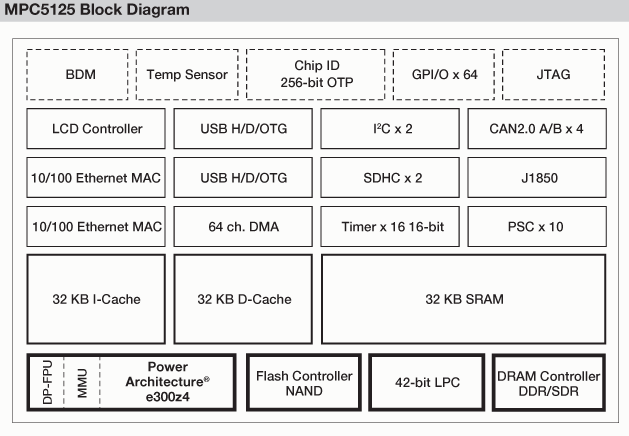
\includegraphics[scale=0.4]{cap3/uproc}
    \caption{Schema a blocchi dell'architettura del microcontrollore MPC5125}
    \label{uproc}
  \end{center}
\end{figure}

Nella Figura \ref{uproc} è presentato lo schema a blocchi del microcontrollore; si può notare la presenza dei dispositivi tipicamente integrati in un prodotto di questa categoria, come ad esempio i GPIO, un modulo JTAG e le DMA.

Il core del microcontrollore è basata su architettura \textit{PowerPC}, ed in particolare si tratta dell'architettura \textit{Power e300z4}. Nel corso di questo paragrafo verrà data una spiegazione più dettagliata di questa architettura.

Infine la scheda integra $256MB$ di memoria RAM e $512MB$ di memoria non volatile, su cui sono caricati i programmi utente ed il sistema operativo.

\subsubsection{Architettura PowerPC}
L'architettura \textit{PowerPC} è nata nel $1991$ dalla collaborazione di \textit{Apple}, \textit{IBM} e \textit{Motorola}. 

La filosofia alla base di questa architettura è denominata RISC (\textit{Reduced Instruction Set Computer}) e prevede lo sviluppo di un processore in grado di eseguire poche istruzioni semplici, per accelerare i tempi di esecuzione. Questa filosofia è nata in contrapposizione alla filosofia CISC (\textit{Complex Instruction Set Computer}) che si era diffusa all'inizio dell'era dell'industria informatica per facilitare il lavoro di sviluppo di programmi, cercando di emulare istruzioni di alto livello, in quanto non erano ancora disponibili i primi compilatori.

Una definizione più precisa delle architetture RISC può essere architettura \textit{load-store}, in quanto le architetture RISC permettono l'accesso alla memoria di sistema unicamente con queste due funzioni.

L'architettura RISC è nata alla fine degli anni $'70$, quando i ricercatori di \textit{IBM} notarono che la maggior parte delle funzioni di indirizzamento integrate nelle ISA (\textit{Instruction Set Architecture}) erano ignorate dai programmatori, a causa dell'introduzione sul mercato dei primi compilatori, che erano in grado di gestire soltanto le istruzioni più semplici dei processori.

Inoltre scoprirono che alcune istruzioni complesse CISC erano più lente del loro corrispettivo sviluppato utilizzando una serie di istruzioni generiche. Per questi motivi si svilupparono set di istruzioni più semplici, che garantissero una progettazione del processore meno complessa e una velocità di esecuzione migliore.
La conseguenza dell'introduzione di questo tipo di architetture è stata la possibilità di sfruttare soluzioni di parallellizzazione delle istruzioni, come la \textit{pipeline}.

\paragraph{PowerPC e300}
L'architettura \textit{e300} comprende una famiglia di processori a $32$-bit sviluppata da \textit{Freescale}, il cui principale utilizzo sono le applicazioni \textit{embedded}.

L'architettura \textit{e300} segue la filosofia RISC precedentemente illustrata ed implementa una pipeline a $4$ stadi. 

L'\textit{e300}, inoltre, segue la filosofia \textit{superscalar}, che prevede la possibilità di leggere dalla memoria e di completare più di un'istruzione per ciclo di clock, aumentando così il \textit{throughput} del sistema.

La pipeline, come accennato sopra, si compone di 4 fasi principali:

\begin{enumerate}
	\item \underline{Fetch}: Si legge l'istruzione da eseguire dalla memoria di sistema e si calcola la posizione dell'istruzione successiva. Inoltre, se necessario, la BPU (\textit{Branch Prediction Unit}) decodifica i branch e decide quale è l'istruzione successiva.
	\item \underline{Dispatch}: Decodifica l'istruzione proveniente dalla fase di fetch e determina quali istruzioni possono essere eseguite nel ciclo corrente. Inoltre gli operatori delle operazioni sono letti dai registri sorgente ed inviati assieme all'istruzione alla fase successiva della pipeline.
	\item \underline{Execution}: In questa fase ogni unità funzionale a cui è stata assegnata un'istruzione esegue l'operazione, scrive il risultato nel registro di destinazione e notifica allo stadio finale della pipeline il termine dell'operazione. In questa fase è possibile che le operazioni richiedano più di un ciclo di clock.
	\item \underline{Complete/write-back}: questa fase si preoccupa di mantenere il corretto comportamento architetturale della macchina, ad esempio in presenza di interrupt la pipeline viene scaricata, i risultati delle precedenti computazioni sono scartati e il flusso di istruzioni viene indirizzato dalla sorgente corretta.
\end{enumerate}

Nella fase di fetch delle istruzioni si è accennato alla presenza di una BPU. Quando si legge dalla memoria un'istruzione di branch non si può sapere a priori quale sarà l'istruzione successiva; la BPU svolge la funzione di effettuare una predizione su quale flusso sarà seguito dal programma ed in caso di successo nella predizione si ottiene come effetto l'assenza di ritardi causati dalla soluzione del branch.

Nell'architettura in esame la predizione della direzione del branch è fatta a \textit{compile time}; all'istruzione di branch è aggiunto un bit che indica la direzione prevista per quel branch e la BPU, che contiene un sommatore al suo interno, è in grado di calcolare l'indirizzo dell'istruzione seguente. Il flusso di istruzioni si mantiene quello della previsione finché il branch non è risolto. A questo punto se la previsione era corretta il flusso di istruzioni viene mantenuto, altrimenti si provvede a scartare i risultati non utili ed il flusso di istruzioni ricomincia seguendo il verso opposto del branch.

Per ulteriori informazioni riguardo l'architettura e il microcontrollore in uso si faccia riferimento al manuale utente, incluso nella bibliografia di questo elaborato \cite{e300manual}.
